\documentclass{article}
\usepackage[utf8]{inputenc}
\usepackage{amsmath}
\usepackage{braket}
\usepackage{gensymb}
\usepackage{amssymb}
\usepackage{natbib}
\usepackage{graphicx}
\usepackage{listings}
\usepackage{color}
\usepackage{tikz}
\usepackage{multicol}
\usetikzlibrary{arrows}
\usepackage{hyperref}
\hypersetup{
    colorlinks=true,
    linkcolor=blue,
    filecolor=magenta,      
    urlcolor=cyan,
}
\usepackage{float}
\restylefloat{figure}

\usepackage[figurename=Figure]{caption}

\definecolor{codegreen}{rgb}{0,0.6,0}
\definecolor{codegray}{rgb}{0.5,0.5,0.5}
\definecolor{codepurple}{rgb}{0.58,0,0.82}
\definecolor{backcolour}{rgb}{0.95,0.95,0.92}
 
\lstdefinestyle{mystyle}{
    backgroundcolor=\color{backcolour},   
    commentstyle=\color{codegreen},
    keywordstyle=\color{magenta},
    numberstyle=\tiny\color{codegray},
    stringstyle=\color{codepurple},
    basicstyle=\footnotesize,
    breakatwhitespace=false,         
    breaklines=true,                 
    captionpos=b,                    
    keepspaces=true,                 
    numbers=left,                    
    numbersep=5pt,                  
    showspaces=false,                
    showstringspaces=false,
    showtabs=false,                  
    tabsize=2
}
 
\lstset{style=mystyle}
\lstset{
    language=Erlang,
    mathescape=true
}

\title{FYS3140 - Home exam 2018}
\author{Candidate: 15028}
\date{April 2018}

\begin{document}

\maketitle

\section*{Problem 1: Differential equation}

We are asked to find the general solution of the differential equation
\begin{equation}
y^{''}(x) + \frac{3}{x}y^{'}(x) - \frac{24}{x^2}y(x) = 56x^6. \label{diff_eq_to_solve}
\end{equation}
Solving this equation involves two major steps; 1) find the complementary function $f_c$, and 2) find the particular solution.
For the complementary function, we start by multiplying through by $x^2$ to get
\begin{equation}
x^2y^{''}(x) + 3xy^{'}(x) - 24y(x) = 56x^8,
\end{equation}
which has the form $ax^2y^{''} + bxy^{y} + cy = g(x)$ and thus is a second order non-homogeneous Cauchy-Euler differential equation.
Reconizing $a = 1, b = 3$ and $c = -24$, we can write 
\begin{equation}
am(m-1) + bm + c = 0 \rightarrow m(m-1) + 3m -24 = m^2 + 2m -24 = 0,
\end{equation}
which yields $m_1 = 4$ and $m_2 = -6$. Since $m_1$ and $m_2$ are two distinct real roots the complementary function is a function on the form
\begin{equation}
y_c = c_1x^{m_1} + c_2x^{m^2} \rightarrow y_c = c_1x^{4} + c_2x^{-6}.
\end{equation}
For the particular solution we will use \textit{variation of parameters}. As we can see, \ref{diff_eq_to_solve} is on the form $y^{''} + p(x)y^{'} + q(x)y = g(x)$. Since $p(x) = 3/x, q(x) = -24/x^2$ and $g(x) = 56x^2$ are all continous on an open interval, the particular solution can be found by
\begin{equation}
Y_p = -y_1\int \frac{y_2g(x)}{W(y_1,y_2)}dx + y_2\int \frac{y_1g(x)}{W(y_1, y_2)}dx,
\end{equation}
where $W(y_1, y_2)$ is the Wronskian of $y_1$ and $y_2$. $y_1$ and $y_2$ is from the complementary function. Starting by finding the Wronskian of $y_1$ and $y_2$
\begin{equation}
W = \begin{vmatrix}y_1&y_2\\y_1^{'}&y_2^{'}\end{vmatrix} \rightarrow W = \begin{vmatrix}x^4&x^{-6}\\4x^3&-6x^{-7}\end{vmatrix} = -6x^{-7}x^4 - 4x^3x^{-6} = -10x^{-3},
\end{equation}
we can write
\begin{align}
Y_p &= -x^4 \int \frac{x^{-6}56x^6}{-10x^{-3}}dx + x^{-6} \int \frac{x^456x^6}{-10x^{-3}}dx \\
 &= \frac{56}{10}\bigg(x^4 \int x^3 \ dx - x^{-6} \int x^{13} \ dx \bigg) \\
 &= \frac{56}{10}\bigg(\frac{x^8}{4} - \frac{x^{8}}{14}\bigg) \\
 &= \frac{56}{10}\bigg(\frac{10x^8}{56}\bigg) \\
 &= x^8
\end{align}
Finnaly, we find our general solution by adding the complementary function and the particular solution togetter
\begin{equation}
y(x) = y_c + Y_P \rightarrow y(x) = c_1x^4 + c_2x^{-6} + x^8,
\end{equation}
which also can be written as
\begin{equation}
y(x) = \frac{c_2}{x^{6}} + c_1x^4 + x^8,
\end{equation}
and that's my final answer.

\section*{Problem 2: Complex analysis}

\subsection*{Part A:}

\subsubsection*{a$)$}

For a function that has a \textit{pole of order 3} at $z = 3 + i$, a \textit{zero of order 4} at $z = 2i$, we have the following function 
\begin{equation}
f(z) = \frac{(z-2i)^4}{(z-[3+i])^3}
\end{equation}

\subsubsection*{b$)$}

We are asked to classify the isolated singularity of the function
\begin{equation}
f(x) = \frac{z^3 + 8}{(z-5)^3(z+2)}.
\end{equation}
If we write
\begin{equation}
f(x) = \frac{1}{(z-5)^3}\frac{z^3+8}{(z+2)}.
\end{equation}
Polynomial division, $(z^3+8):(z+2)$, yields
\begin{equation}
f(x) = \frac{z^2 - 2z + 4}{(z-5)^3},
\end{equation}
which shows $z = -2$ is a \textit{removable singularity}. Now, if we write
\begin{align}
\frac{1}{(z-5)^3} &= \bigg(\frac{1}{z-5}\bigg)^3 = \bigg(-\frac{\frac{1}{5}}{1-\frac{z}{5}}\bigg)^3 \\
 &= \bigg(-\frac{1}{5}\frac{1}{1-\frac{z}{5}}\bigg)^3 = \bigg(-\frac{1}{5}\sum_{n=0}^{\infty}\big(\frac{z}{5}\big)^n\bigg)^3 \\
 &= \bigg(-\frac{1}{5}\bigg[1 + \frac{z}{5} + \frac{z^2}{25} + \frac{z^3}{25} + ... \bigg]\bigg)^3 \\
 &= \bigg(-\frac{1}{5} - \frac{z}{25} - \frac{z^2}{125} - \frac{z^3}{675} + ...\bigg)^3
\end{align}


\subsection*{Part B:}

\subsubsection*{a$)$}
We start writing $\cot{(z)}$ as $\cos{(z)}/\sin{(z)}$ to get
\begin{equation}
g(z) = f(z)\pi\cot{(\pi z)} = \frac{f(z)\pi\cos{(\pi z)}}{\sin{(\pi z)}}.
\end{equation}
If we now set $a(z) \equiv f(z)\pi\cos{\pi z}$ and $b(z) \equiv \sin{\pi z}$ we have that $g(z) = a(z)/b(z)$, $a(n) = \text{finite constant} \neq 0$, and $b(n) = 0$, $b^{'}(n) \neq 0$ and thus the residue can be found by equation $6.2$ in Boas
\begin{equation}
Res(n) = \frac{a(n)}{b^{'}(n)} \rightarrow Res(n) = \frac{f(n)\pi\cos(\pi n)}{\pi\cos(\pi n)} = f(n),
\end{equation}
which is what we were suppose to show.
\subsubsection*{b$)$}
$N = 1/2$ yields $K = 1$, so let's go for that! With $K = 1$, we get the following contour
\begin{figure}[H]
\centering
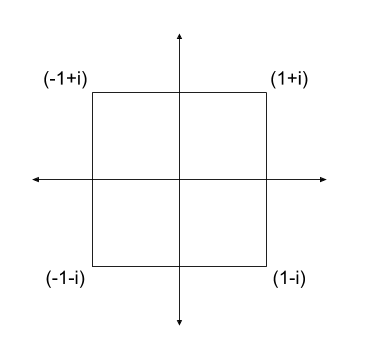
\includegraphics[width=0.6\textwidth]{complex_contour}
\caption{Contour for $N=1/2$.}
\label{fig:figure_label}
\end{figure}




\subsubsection*{c$)$}

\subsubsection*{d$)$}

\section*{Problem 3: The Dirac delta function}

\subsection*{a$)$}

% solution:
%https://math.stackexchange.com/questions/959178/proof-of-an-identity-of-the-dirac-delta

We will use two usefull identeties in this proof;
\begin{equation}
\int_a^b \delta(t)g(x) = \begin{cases}0 &: \not\in (a, b) \\ g(x) &: \in (a,b)\end{cases} \label{delta_ref_1}.
\end{equation}
\begin{equation}
\int_a^b \delta(ft)g(x) = \frac{1}{|x|}\int\delta(x)g(x)dx \label{delta_ref_2}
\end{equation}
We start by using the hint and introduce an arbitrary test funciton $g(t)$. Taking the intergal of this yields
\begin{equation}
\int_{-\infty}^{+\infty} \delta[f(x)]g(t)dt,
\end{equation}
which can be written as a sum of three intergrals
\begin{equation}
\int_{-\infty}^{t_0-\epsilon} \delta[f(t)]g(t)dt + \int_{t_0-\epsilon}^{t_0 + \epsilon} \delta[f(t)]g(t)dt + \int_{t_0 + \epsilon}^{+\infty} \delta[f(t)]g(t)dt.
\end{equation}
By the definition of the delta function, we know that $f(t)$ only have a zero in the middle term and thus the first and last integral is zero which yields
\begin{equation}
\int_{-\infty}^{+\infty} \delta[f(t)]g(t)dt = \int_{t_0-\epsilon}^{t_0 + \epsilon} \delta[f(t)]g(t)dt.
\end{equation}
Expanding $f(t)$ centered at $t_0$ up to the first order yields $f(t_0) + f'(t_0)(t - t_0)$ and thus, with $f(t_0) = 0$, we have
\begin{equation}
\int_{-\infty}^{+\infty} \delta[f(t)]g(t)dt = \int_{t_0-\epsilon}^{t_0 + \epsilon} \delta[f'(t_0)(t-t_0)]g(t)dt 
\end{equation}
By \ref{delta_ref_2}, we can write
\begin{equation}
\int_{-\infty}^{+\infty} \delta[f(t)]g(t)dt = \frac{1}{|f'(t_0)|} \int_{t_0-\epsilon}^{t_0 + \epsilon} \delta(t-t_0)g(t)dt 
\end{equation}
On a generalized form we can summarize over all $t_i$ which yields

\begin{equation}
\int_{-\infty}^{+\infty} \delta[f(t)]g(t)dt = \sum_{i}\frac{1}{|f'(t_i)|} \int_{t_i-\epsilon}^{t_i + \epsilon} \delta(t-t_i)g(t)dt 
\end{equation}

\subsection*{b$)$}

\subsubsection*{(i)}
For $f(t) = t^2 -a^2$ we have $f'(t) = 2t \rightarrow f'(a) = 2a, \ f'(-a) = -2a$ yielding
\begin{equation}
\delta(t^2 - a^2) = \delta((t+a)(t-a)) = \sum_{i} \frac{\delta(t-t_i)}{|2t|} = \frac{1}{2a}\delta(t-a) + \frac{1}{2a}\delta(t+a)
\end{equation}

\subsubsection*{(i)}
For $f(t) = \sin(t)$ we have $f'(t) = cos(t) \rightarrow f'(0) = 1 \ f'(\pi) = -1$
\begin{equation}
\delta(\sin{(t)}) = \sum_{i} \frac{\delta(t-t_i)}{|cos(t)|} = \delta(t-0) +\delta(t+\pi)
\end{equation}


\subsection*{c$)$}

\begin{figure}[H]
\centering
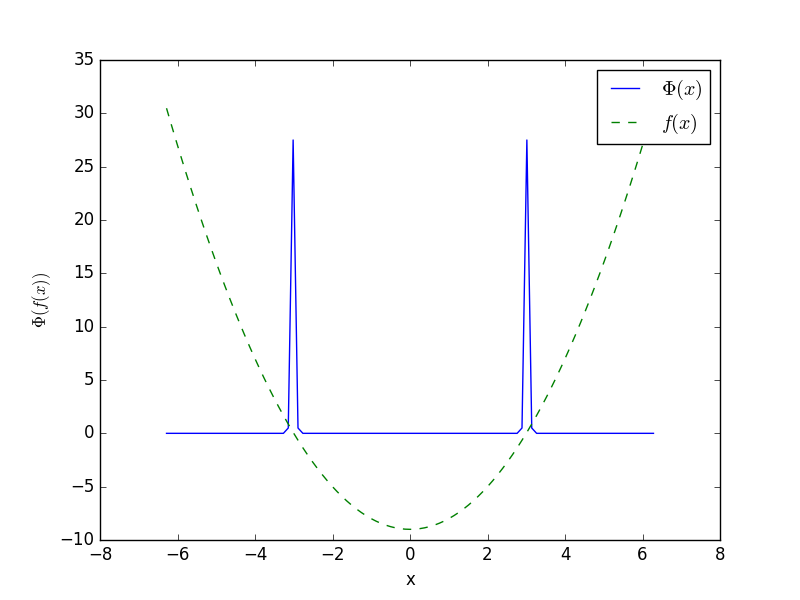
\includegraphics[width=0.6\textwidth]{matmet_figure_1}
\caption{As expected we see two peeks at the roots $a \pm 3$.}
\label{fig:figure_label}
\end{figure}

\begin{figure}[H]
\centering
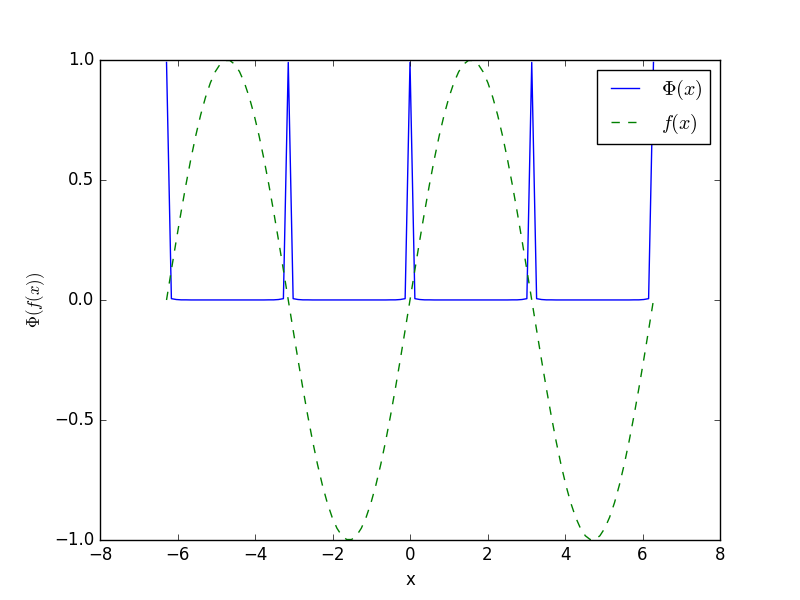
\includegraphics[width=0.6\textwidth]{matmet_figure_2}
\caption{As expected we see periodical peeks at $n = 0, \pi, 2\pi, ...$.}
\label{fig:figure_label}
\end{figure}

\subsection*{d$)$}
We start with the integral
\begin{equation}
\int_{-\pi/2}^{+\pi/2}\cos{t}\delta{[\sin{t}]}dt,
\end{equation}
which can we written as
\begin{equation}
\int_{-\pi/2}^{+\pi/2}\cos{t}\sum_{i} \frac{\delta(t-t_i)}{|\cos{t_i}|} dt.
\end{equation}
We are integrating from $-\pi/2$ to $\pi/2$. In this interval, $\sin{t}$ is only zero at $t=0$ which yields
\begin{equation}
\int_{-\pi/2}^{+\pi/2}\cos{t} \frac{\delta(t)}{|\cos{0}|} dt = \int_{-\pi/2}^{+\pi/2}\cos{t}\delta(t) dt = 1.
\end{equation}



\end{document}

